%!TEX root = ../thesis.tex
\section{要求仕様}
本研究では,QDD(Quasi-Direct Drive)モータを搭載したロボットアームを開発し,オフィス環境での作業遂行を目指す.そのため,以下の要求仕様を策定する.これらの仕様は,設定した作業内容や既存のオフィスロボットの調査結果を基に決定したものである.特に,QDDモータを採用することで,柔軟性と安全性を高める点に注力している.

\subsection{サイズと作業範囲}
ロボットアームのサイズは,机上での片付け作業を想定し,50cm以内の範囲にある対象物を扱えるよう設計する.これを実現するため,アームのリーチは70cm程度とする.この範囲は既存のロボットアームの調査結果を基準として設定したものであり,オフィス環境における机上作業の多くをカバーできる.

\subsection{自由度}
自由度の決定は既存のオフィスロボットを参考に行う.既存のオフィスロボットの自由度を調査した結果を示す.7自由度と6自由度のロボットがほとんどである.6自由度に比べ7自由度は柔軟な操作が可能であるが,アーム重量が増加し,コストも高くなるため,6自由度を採用する.軸配置についても既存のロボットアームを参考に,肩2軸(ヨー,ピッチ),肘1軸(ロール),手首3軸(ヨー,ピッチ,ロール)とする.

\begin{figure}[h]
  \centering
  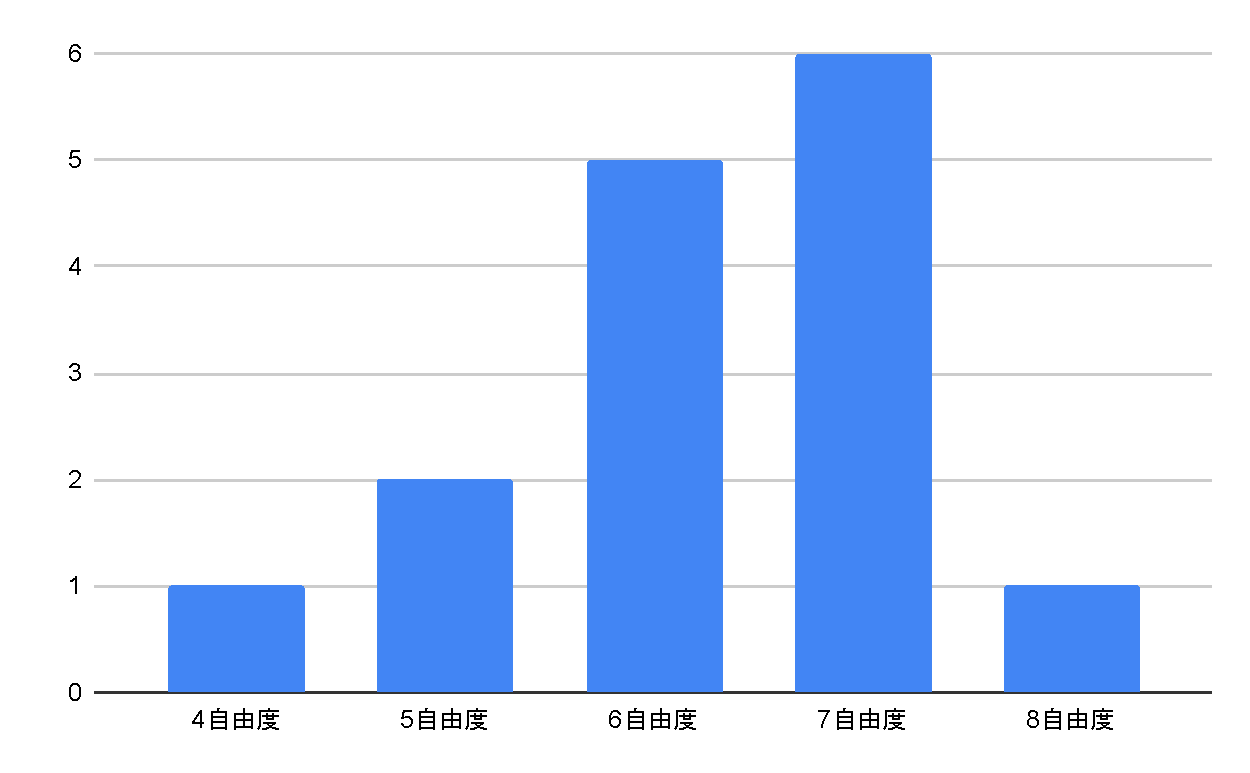
\includegraphics[width=10cm]{images/armDof.pdf}
  \caption{Existing office robot arm DoF}
  \label{fig:armDof}
\end{figure}

\subsection{可搬重量}
オフィス環境での作業では軽量な物体を扱うことが多く,設定した作業では500g以下の物体を対象とした.そのため,アームの可搬重量は500g以上の可搬重量を確保する.これにより,オフィス作業で想定される軽量物の取り扱いを十分にカバーできる.
\subsection{エンドエフェクタ}
既存のオフィスロボットのエンドエフェクタは,Mobile ALOHAに搭載されているロボットアーム(\ref{fig:alohaarm}に示す)のような平行グリッパが多く,様々な形状の物体を把持していることが確認できた.そのため,本研究で開発するアームにも平行グリッパを搭載する.

\begin{figure}[h]
  \centering
  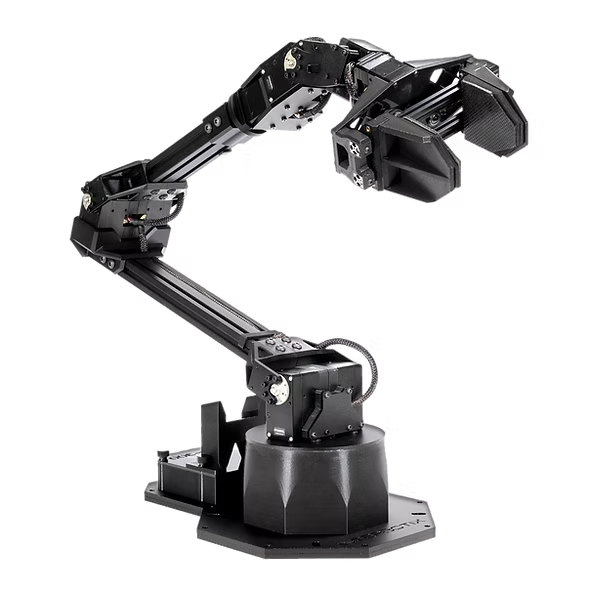
\includegraphics[width=10cm]{images/alohaarm.png}
  \caption{Mobile ALOHO Arm}
  \label{fig:alohaarm}
\end{figure}

\subsection{安全性}
人や精密機器があるオフィス環境では、ロボットがそれらの危害を加えないことが最も重要である.接触してしまっても,ロボットアームの関節が柔軟に駆動すれば被害は最小限に抑えることができると考られるため,QDDモータを使用する.QDDモータは低減速比でバックドライバビリティが高いため,人や機器との衝撃を最小限に抑え,オフィス環境での安全性に寄与する.
\subsection{オープンプラットフォーム}
開発するロボットアームはオープンプラットフォームオフィスロボットの一部機能であるため,オープンプラットフォームであることが望ましい.オープンプラットフォームとして,以下の項目を満たすことが望ましい.
\begin{itemize}
  \item ハードウェアの設計図の公開
  \item 部品リストの公開
  \item 製作動画の公開
\end{itemize}

\section{要求仕様のまとめ}
以上の項目をまとめた要求仕様を表\ref{tab:armSpecs}に示す.これらの項目を満たしたロボットアームを設計する.

\begin{table}
  \centering
  \begin{tabular}{l|l}
    \hline
    \multicolumn{1}{c|}{\textbf{項目}} & \multicolumn{1}{c}{\textbf{仕様}} \\ \hline
    アームリーチ                           & 約70cm                           \\
    自由度                              & 6自由度                            \\
    可搬重量                             & 500g以上                          \\
    エンドエフェクタ                         & 平行グリッパ                          \\
    安全性                              & QDDモータを使用した柔軟な関節                \\
    オープンプラットフォーム性                    & 設計データおよび製作ノウハウの公開               \\ \hline
  \end{tabular}
  \caption{Required specifications for robot arm}
  \label{tab:armSpecs}
\end{table}
\clearpage
\newpage